\documentclass[12pt, a4paper]{article}

% ── Packages ──────────────────────────────────────────────
\usepackage[margin=1in]{geometry}
\usepackage{amsmath, amssymb}
\usepackage{graphicx}
\usepackage{booktabs}
\usepackage{hyperref}
\usepackage{enumitem}
\usepackage{algorithm}
\usepackage{algpseudocode}
\usepackage{xcolor}
\usepackage{listings}
\usepackage{caption}
\usepackage{subcaption}
\usepackage{tikz}
\usetikzlibrary{arrows.meta, positioning, shapes.geometric, fit}
\usepackage{float}

\hypersetup{
    colorlinks=true,
    linkcolor=blue!70!black,
    citecolor=green!50!black,
    urlcolor=blue!60!black,
}

\lstset{
    language=Python,
    basicstyle=\ttfamily\small,
    keywordstyle=\color{blue!70!black}\bfseries,
    commentstyle=\color{green!50!black}\itshape,
    stringstyle=\color{red!60!black},
    frame=single,
    breaklines=true,
    numbers=left,
    numberstyle=\tiny\color{gray},
}

% ── Title ─────────────────────────────────────────────────
\title{%
    \textbf{Adversarial Image Detection via Feature Consistency\\
    in Vision Transformers}\\[0.5em]
    \large A Two-Model Transfer-Attack Detection Framework
}
\author{
    Machine Learning Sessional Project Report
}
\date{\today}

\begin{document}
\maketitle

\begin{abstract}
    We present a framework for detecting adversarial images by exploiting
    the \emph{feature consistency} property of Vision Transformers (ViTs).
    The system employs a two-model architecture: a fine-tuned ResNet-18
    serves as the attack target model for crafting adversarial perturbations
    (via FGSM and PGD), while a pretrained ViT-B/16 acts as the detection
    model by extracting intermediate transformer-block features. We
    construct a 24-dimensional \emph{feature consistency score vector} by
    measuring how ViT's internal representations shift under benign
    transformations (Gaussian blur, Gaussian noise, and rotation). A
    meta-classifier trained on these score vectors distinguishes clean
    images from adversarial ones. Evaluated on CIFAR-100 with 100 test
    images (300 total samples: clean + FGSM + PGD), our detector achieves
    \textbf{99.0\% accuracy} (297/300 correct). Additionally, we analyze
    the ViT representation shift under transfer attacks, finding that FGSM
    shifts ViT's own predictions 55.0\% of the time and PGD shifts them
    48.0\% of the time, confirming the cross-architecture transferability
    of adversarial perturbations.
\end{abstract}

\tableofcontents
\newpage

% ══════════════════════════════════════════════════════════
\section{Introduction}
% ══════════════════════════════════════════════════════════

Deep neural networks are vulnerable to \emph{adversarial examples}---inputs
with small, carefully crafted perturbations that cause models to
misclassify with high confidence \cite{goodfellow2015explaining,
madry2018towards}. This vulnerability raises serious concerns for
safety-critical applications such as autonomous driving, medical imaging,
and security systems.

Most adversarial defense research focuses on making models \emph{robust}
to attacks (adversarial training) or on detecting adversarial inputs
before they reach the classifier. Our work falls into the latter
category: we build a detector that identifies adversarial images
\emph{without modifying} the target classifier.

\subsection{Key Idea: Feature Consistency}

The central insight of this project is that \textbf{clean images exhibit
stable (consistent) internal representations under small benign
transformations}, whereas \textbf{adversarial images exhibit unstable
(inconsistent) representations}. Adversarial perturbations are finely
tuned to exploit specific model vulnerabilities; even minor
transformations (a slight blur, a small rotation, or low-level noise) can
disrupt the adversarial pattern, causing significant shifts in the
model's internal feature space.

We leverage the intermediate transformer-block features of a pretrained
Vision Transformer (ViT-B/16) to measure this consistency and train a
lightweight meta-classifier to distinguish clean from adversarial images.

\subsection{Two-Model Architecture}

Our framework deliberately uses \emph{two different architectures}:
\begin{itemize}[nosep]
    \item \textbf{Attack Model (ResNet-18, CNN):} Generates adversarial
          examples via gradient-based attacks (FGSM, PGD).
    \item \textbf{Detection Model (ViT-B/16, Transformer):} Extracts
          intermediate features for consistency analysis.
\end{itemize}

This creates a realistic \emph{transfer-attack} scenario: adversarial
perturbations are crafted against a CNN but must fool a Transformer-based
detector---a significantly harder task due to architectural differences
in how CNNs and Transformers process visual information.

% ══════════════════════════════════════════════════════════
\section{Background and Theory}
% ══════════════════════════════════════════════════════════

\subsection{Adversarial Examples}

Given a classifier $f_\theta$ with parameters $\theta$, an input image
$\mathbf{x}$ with true label $y$, and a loss function
$\mathcal{L}(\theta, \mathbf{x}, y)$, an adversarial example
$\mathbf{x}_{\mathrm{adv}}$ satisfies:
\begin{equation}
    f_\theta(\mathbf{x}_{\mathrm{adv}}) \neq y
    \quad \text{subject to} \quad
    \|\mathbf{x}_{\mathrm{adv}} - \mathbf{x}\|_\infty \leq \epsilon
\end{equation}
where $\epsilon$ is the perturbation budget. The perturbation
$\delta = \mathbf{x}_{\mathrm{adv}} - \mathbf{x}$ is typically
imperceptible to humans.

\subsection{Fast Gradient Sign Method (FGSM)}

FGSM \cite{goodfellow2015explaining} computes the adversarial example in
a single gradient step:
\begin{equation}
    \mathbf{x}_{\mathrm{adv}} = \mathbf{x} + \epsilon \cdot
    \mathrm{sign}\!\left(\nabla_{\mathbf{x}}
    \mathcal{L}(\theta, \mathbf{x}, y)\right)
\end{equation}

This is a fast, single-step attack that perturbs each pixel by exactly
$\pm\epsilon$ in the direction that maximizes the classification loss.
In our implementation, we use $\epsilon = 8/255 \approx 0.031$.

\subsection{Projected Gradient Descent (PGD)}

PGD \cite{madry2018towards} is an iterative extension of FGSM that
applies multiple smaller steps while projecting back into the
$\epsilon$-ball:
\begin{equation}
    \mathbf{x}^{(t+1)} = \Pi_{\mathbf{x}, \epsilon}\!\left(
    \mathbf{x}^{(t)} + \alpha \cdot \mathrm{sign}\!\left(
    \nabla_{\mathbf{x}^{(t)}}
    \mathcal{L}(\theta, \mathbf{x}^{(t)}, y)\right)\right)
\end{equation}
where $\Pi_{\mathbf{x}, \epsilon}$ projects the result back into the
$\ell_\infty$-ball of radius $\epsilon$ around the original image
$\mathbf{x}$, and $\alpha$ is the step size per iteration. We use
$\epsilon = 8/255$, $\alpha = 2/255$, and 7 iterations.  PGD starts from
a random point within the $\epsilon$-ball, making it stronger than FGSM.

\subsection{Vision Transformer (ViT)}

The Vision Transformer \cite{dosovitskiy2021image} processes an image by:
\begin{enumerate}[nosep]
    \item Splitting it into $16 \times 16$ non-overlapping patches.
    \item Linearly projecting each patch into a $D$-dimensional embedding
          (for ViT-B/16, $D = 768$).
    \item Prepending a learnable \texttt{[CLS]} token.
    \item Adding positional embeddings.
    \item Passing through $L = 12$ transformer encoder blocks, each
          containing multi-head self-attention (MSA) and an MLP.
\end{enumerate}

For an input image of size $224 \times 224$, the patch sequence has
length $196 + 1 = 197$ (196 patch tokens + 1 \texttt{[CLS]} token). Each
transformer block outputs a tensor of shape
$(B, 197, 768)$.

The \texttt{[CLS]} token at the output of each block serves as a global
representation of the image at that layer's level of abstraction. We
extract the \texttt{[CLS]} token from blocks 3, 6, 9, and 11 (0-indexed)
to capture features at different depths.

\subsection{Feature Consistency Hypothesis}

Let $\phi_l(\mathbf{x})$ denote the \texttt{[CLS]} token feature
extracted from ViT block $l$ for input $\mathbf{x}$, and let
$T(\mathbf{x})$ represent a benign transformation of $\mathbf{x}$.

\begin{itemize}
    \item \textbf{Clean images:}
    $d\bigl(\phi_l(\mathbf{x}),\;\phi_l(T(\mathbf{x}))\bigr)$
    is \emph{small}, because benign transformations do not significantly
    alter the semantic content.

    \item \textbf{Adversarial images:}
    $d\bigl(\phi_l(\mathbf{x}_{\mathrm{adv}}),\;
    \phi_l(T(\mathbf{x}_{\mathrm{adv}}))\bigr)$
    is \emph{large}, because even small transformations can disrupt the
    carefully crafted adversarial perturbation, causing large feature
    shifts.
\end{itemize}

where $d(\cdot, \cdot)$ is a distance metric (L2 or cosine distance).

% ══════════════════════════════════════════════════════════
\section{System Architecture}
% ══════════════════════════════════════════════════════════

Figure~\ref{fig:architecture} illustrates the complete system pipeline.

\begin{figure}[H]
\centering
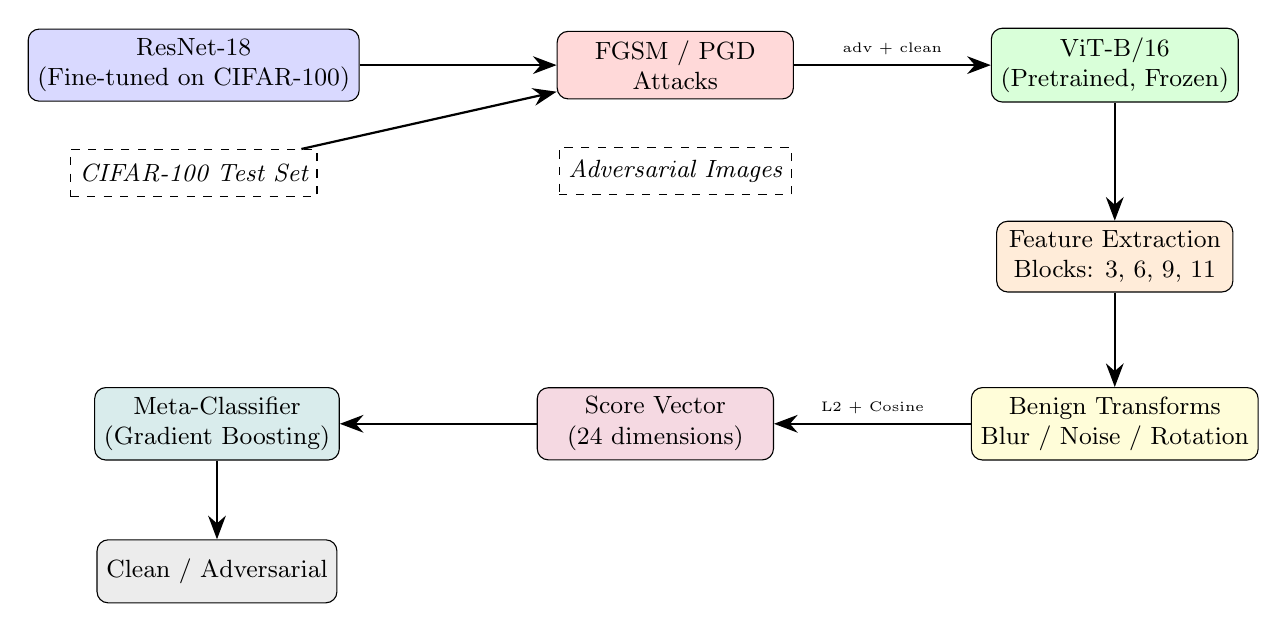
\begin{tikzpicture}[
    node distance=1.2cm and 1.5cm,
    block/.style={rectangle, draw, rounded corners, minimum width=3cm,
                  minimum height=0.8cm, align=center, font=\small},
    arrow/.style={-{Stealth[length=3mm]}, thick},
    data/.style={rectangle, draw, dashed, minimum width=2.5cm,
                 minimum height=0.6cm, align=center, font=\small\itshape},
]
    % Phase 1
    \node[block, fill=blue!15] (resnet) {ResNet-18\\(Fine-tuned on CIFAR-100)};
    \node[data, below=0.6cm of resnet] (cifar) {CIFAR-100 Test Set};
    
    % Phase 2 - Attacks
    \node[block, fill=red!15, right=2.5cm of resnet] (attacks) {FGSM / PGD\\Attacks};
    \node[data, below=0.6cm of attacks] (advimg) {Adversarial Images};
    
    % Phase 3 - ViT
    \node[block, fill=green!15, right=2.5cm of attacks] (vit) {ViT-B/16\\(Pretrained, Frozen)};
    
    % Phase 4 - Features
    \node[block, fill=orange!15, below=1.5cm of vit] (features) {Feature Extraction\\Blocks: 3, 6, 9, 11};
    
    % Phase 5 - Transforms
    \node[block, fill=yellow!15, below=1.2cm of features] (transforms) {Benign Transforms\\Blur / Noise / Rotation};
    
    % Phase 6 - Score Vector
    \node[block, fill=purple!15, left=2.5cm of transforms] (score) {Score Vector\\(24 dimensions)};
    
    % Phase 7 - Meta Classifier
    \node[block, fill=teal!15, left=2.5cm of score] (meta) {Meta-Classifier\\(Gradient Boosting)};
    
    % Output
    \node[block, fill=gray!15, below=1.0cm of meta] (output) {Clean / Adversarial};
    
    % Arrows
    \draw[arrow] (resnet) -- (attacks);
    \draw[arrow] (cifar) -- (attacks);
    \draw[arrow] (attacks) -- (vit) node[midway, above, font=\tiny] {adv + clean};
    \draw[arrow] (vit) -- (features);
    \draw[arrow] (features) -- (transforms);
    \draw[arrow] (transforms) -- (score) node[midway, above, font=\tiny] {L2 + Cosine};
    \draw[arrow] (score) -- (meta);
    \draw[arrow] (meta) -- (output);
\end{tikzpicture}
\caption{System architecture overview: from adversarial generation to detection.}
\label{fig:architecture}
\end{figure}

\subsection{Module Descriptions}

The project is organized into the following modules:

\begin{table}[H]
\centering
\caption{Project module structure and responsibilities.}
\label{tab:modules}
\begin{tabular}{@{}ll@{}}
\toprule
\textbf{Module} & \textbf{Responsibility} \\
\midrule
\texttt{models/resnet\_loader.py} & Load/fine-tune ResNet-18 for CIFAR-10/100 \\
\texttt{models/vit\_loader.py}    & Load pretrained ViT-B/16 with forward hooks \\
\texttt{attacks/fgsm.py}          & FGSM adversarial attack implementation \\
\texttt{attacks/pgd.py}           & PGD adversarial attack implementation \\
\texttt{features/feature\_extractor.py} & Extract CLS token features from ViT blocks \\
\texttt{features/feature\_distance.py}  & Compute L2 and cosine distance score vectors \\
\texttt{utils/transforms.py}      & Benign transformations (blur, noise, rotation) \\
\texttt{dataset/build\_score\_dataset.py} & Build labeled score dataset (clean vs.\ adversarial) \\
\texttt{meta\_model/train\_classifier.py} & Train and evaluate meta-classifiers \\
\texttt{meta\_model/inference\_classifier.py} & End-to-end inference pipeline \\
\texttt{main.py}                   & CLI entry point with subcommands \\
\bottomrule
\end{tabular}
\end{table}

% ══════════════════════════════════════════════════════════
\section{Methodology}
% ══════════════════════════════════════════════════════════

\subsection{Phase 1: Fine-Tuning ResNet-18 on CIFAR-100}

\textbf{Purpose:} Create a competent classifier that can be attacked
with meaningful gradient-based adversarial perturbations.

\textbf{Architecture Modifications for CIFAR-100:}
\begin{itemize}[nosep]
    \item Replace the first $7 \times 7$ convolution (designed for
          $224 \times 224$ ImageNet images) with a $3 \times 3$
          convolution for $32 \times 32$ CIFAR images.
    \item Remove the max-pooling layer (replaced with identity) to
          preserve spatial resolution.
    \item Replace the final fully connected layer:
          $\text{Linear}(512, 1000) \rightarrow \text{Linear}(512, 100)$.
\end{itemize}

\textbf{Training Configuration:}
\begin{table}[H]
\centering
\caption{ResNet-18 fine-tuning hyperparameters.}
\begin{tabular}{@{}ll@{}}
\toprule
\textbf{Parameter} & \textbf{Value} \\
\midrule
Dataset       & CIFAR-100 (training split, 50{,}000 images) \\
Epochs        & 25 \\
Batch Size    & 128 \\
Optimizer     & Adam ($\text{lr} = 0.001$) \\
Scheduler     & Cosine Annealing \\
Loss Function & Cross-Entropy \\
Augmentation  & Random Crop (32, padding=4) + Random Horizontal Flip \\
\bottomrule
\end{tabular}
\end{table}

\textbf{Why fine-tuning is necessary:}
A well-trained classifier produces strong, meaningful gradients during
adversarial attacks. Without fine-tuning, the model's poor accuracy on
CIFAR-100 ($\sim$1\% random chance for 100 classes) would yield weak,
noisy perturbations that do not represent realistic adversarial threats.
The meta-classifier would then learn to detect noise rather than true
adversarial patterns, leading to poor generalization.

\subsection{Phase 2: Building the Feature Consistency Score Dataset}

This phase constructs the training data for the meta-classifier. For each
image from the CIFAR-100 \textbf{test set}, we generate three samples:

\begin{enumerate}[nosep]
    \item \textbf{Clean sample} (label = 0): Compute score vector from
          the original image.
    \item \textbf{FGSM adversarial sample} (label = 1): Attack the image
          via ResNet-18 with FGSM, then compute its score vector.
    \item \textbf{PGD adversarial sample} (label = 1): Attack the image
          via ResNet-18 with PGD, then compute its score vector.
\end{enumerate}

\textbf{Why we use the test set (not training set):}
ResNet-18 was fine-tuned on the CIFAR-100 \emph{training} set. If we
generated adversarial examples from training images, the attacks would
exploit memorized features rather than learned decision boundaries. Using
the test set ensures:
\begin{itemize}[nosep]
    \item Adversarial attacks exploit genuine model vulnerabilities.
    \item The meta-classifier learns generalizable detection patterns.
    \item Results reflect realistic deployment scenarios.
\end{itemize}

\subsubsection{Score Vector Construction}

For each image (clean or adversarial), the 24-dimensional score vector is
computed as follows:

\begin{algorithm}[H]
\caption{Compute Feature Consistency Score Vector}
\label{alg:score}
\begin{algorithmic}[1]
\Require Image $\mathbf{x}$, ViT model with hooks on blocks
$\{3, 6, 9, 11\}$
\Ensure Score vector $\mathbf{s} \in \mathbb{R}^{24}$

\State $\mathbf{s} \gets []$
\State $\mathbf{f}_{\mathrm{orig}} \gets \text{ExtractCLS}(\text{ViT},
\mathbf{x})$
\Comment{CLS tokens from blocks 3, 6, 9, 11}

\For{$T \in \{\text{GaussianBlur},\; \text{GaussianNoise},\;
\text{Rotation}\}$}
    \State $\tilde{\mathbf{x}} \gets T(\mathbf{x})$
    \State $\mathbf{f}_{\mathrm{trans}} \gets
    \text{ExtractCLS}(\text{ViT}, \tilde{\mathbf{x}})$
    
    \For{$l \in \{3, 6, 9, 11\}$}
        \State $\mathbf{s}.\text{append}\!\left(
        \|\mathbf{f}_{\mathrm{orig}}^{(l)} -
        \mathbf{f}_{\mathrm{trans}}^{(l)}\|_2\right)$
        \Comment{L2 distance}
    \EndFor
    \For{$l \in \{3, 6, 9, 11\}$}
        \State $\mathbf{s}.\text{append}\!\left(
        1 - \cos\!\left(\mathbf{f}_{\mathrm{orig}}^{(l)},\;
        \mathbf{f}_{\mathrm{trans}}^{(l)}\right)\right)$
        \Comment{Cosine distance}
    \EndFor
\EndFor

\State \Return $\mathbf{s}$
\Comment{$|\mathbf{s}| = 3 \times 4 \times 2 = 24$}
\end{algorithmic}
\end{algorithm}

\textbf{Score vector layout (24 dimensions):}

\begin{table}[H]
\centering
\caption{Layout of the 24-dimensional feature consistency score vector.}
\label{tab:score_layout}
\small
\begin{tabular}{@{}clcc@{}}
\toprule
\textbf{Index} & \textbf{Description} & \textbf{Transform} & \textbf{Metric} \\
\midrule
0--3   & Blur, Blocks 3/6/9/11    & Gaussian Blur   & L2     \\
4--7   & Blur, Blocks 3/6/9/11    & Gaussian Blur   & Cosine \\
8--11  & Noise, Blocks 3/6/9/11   & Gaussian Noise  & L2     \\
12--15 & Noise, Blocks 3/6/9/11   & Gaussian Noise  & Cosine \\
16--19 & Rotation, Blocks 3/6/9/11 & Rotation (5\textdegree) & L2 \\
20--23 & Rotation, Blocks 3/6/9/11 & Rotation (5\textdegree) & Cosine \\
\bottomrule
\end{tabular}
\end{table}

\textbf{Benign transformation parameters:}
\begin{itemize}[nosep]
    \item Gaussian Blur: kernel size = 3, $\sigma = 0.5$
    \item Gaussian Noise: $\sigma = 0.02$
    \item Rotation: $5°$ fixed angle
\end{itemize}

These transformations are intentionally mild. They barely affect ViT's
perception of clean images but significantly disrupt adversarial
perturbations.

\subsection{Phase 3: Training the Meta-Classifier}

The score dataset is split 80/20 (stratified by class) into training and
test sets.  Features are standardized using \texttt{StandardScaler}.
Four classifiers are trained:

\begin{table}[H]
\centering
\caption{Meta-classifier models and configurations.}
\label{tab:classifiers}
\begin{tabular}{@{}ll@{}}
\toprule
\textbf{Model} & \textbf{Configuration} \\
\midrule
Logistic Regression  & max\_iter = 1000 \\
Random Forest        & 100 estimators \\
Gradient Boosting    & 100 estimators \\
MLP                  & Hidden layers: (64, 32), early stopping \\
\bottomrule
\end{tabular}
\end{table}

The best model is selected based on the highest ROC-AUC score on the test
split and saved for deployment.

\textbf{Evaluation metrics:} Accuracy, Precision, Recall, F1-score, and
ROC-AUC.

\subsection{Phase 4: Inference and Demo}

During inference, for a given input image:
\begin{enumerate}[nosep]
    \item Compute the 24-dimensional score vector using the frozen ViT.
    \item Standardize the vector using the saved scaler.
    \item Predict with the saved meta-classifier.
    \item Output: \texttt{CLEAN IMAGE} or \texttt{ADVERSARIAL IMAGE} with
          confidence.
\end{enumerate}

The demo additionally:
\begin{itemize}[nosep]
    \item Generates FGSM and PGD attacks on-the-fly against ResNet-18.
    \item Measures \emph{ViT representation shift}: whether the ViT's own
          ImageNet classification changes from the clean image to the
          adversarial image, quantifying cross-architecture attack
          transferability.
\end{itemize}

% ══════════════════════════════════════════════════════════
\section{Experimental Configuration}
% ══════════════════════════════════════════════════════════

\subsection{Execution Pipeline}

The experiment was executed with the following commands:

\begin{lstlisting}[language=bash, caption={Execution commands for the CIFAR-100 experiment.}]
python main.py finetune-resnet --dataset cifar100   # Step 1
python main.py build-dataset --dataset cifar100     # Step 2
python main.py train                                # Step 3
python main.py demo --dataset cifar100              # Step 4
\end{lstlisting}

\subsection{Configuration Summary}

\begin{table}[H]
\centering
\caption{Complete experimental configuration.}
\begin{tabular}{@{}lll@{}}
\toprule
\textbf{Component} & \textbf{Parameter} & \textbf{Value} \\
\midrule
\multirow{2}{*}{Dataset}
    & Name      & CIFAR-100 \\
    & Classes   & 100 \\
\midrule
\multirow{3}{*}{Attack Model}
    & Architecture & ResNet-18 (modified for 32$\times$32) \\
    & Training     & Fine-tuned on CIFAR-100 train split \\
    & Epochs       & 25 \\
\midrule
\multirow{3}{*}{Detection Model}
    & Architecture  & ViT-B/16 (from \texttt{timm}) \\
    & Weights       & ImageNet pretrained (frozen) \\
    & Hooked blocks & 3, 6, 9, 11 \\
\midrule
\multirow{2}{*}{FGSM Attack}
    & $\epsilon$  & $8/255 \approx 0.031$ \\
\midrule
\multirow{3}{*}{PGD Attack}
    & $\epsilon$  & $8/255$ \\
    & $\alpha$    & $2/255$ \\
    & Steps       & 7 \\
\midrule
\multirow{3}{*}{Score Vector}
    & Dimensions   & 24 \\
    & Transforms   & Blur, Noise, Rotation \\
    & Metrics      & L2 distance, Cosine distance \\
\midrule
\multirow{2}{*}{Meta-Classifier}
    & Models tested & LR, RF, GB, MLP \\
    & Selection     & Best ROC-AUC \\
\midrule
\multirow{2}{*}{Demo}
    & Test images   & 100 (from CIFAR-100 test set) \\
    & Total samples & 300 (100 clean + 100 FGSM + 100 PGD) \\
\bottomrule
\end{tabular}
\end{table}

% ══════════════════════════════════════════════════════════
\section{Results}
% ══════════════════════════════════════════════════════════

\subsection{Detection Accuracy}

The meta-classifier was evaluated on 100 test images from the CIFAR-100
test set.  For each image, three predictions were made: one for the
clean version, one for the FGSM-attacked version, and one for the
PGD-attacked version, yielding 300 total predictions.

\begin{table}[H]
\centering
\caption{Detection results on CIFAR-100 (100 images, 300 total samples).}
\label{tab:results}
\begin{tabular}{@{}lcc@{}}
\toprule
\textbf{Metric} & \textbf{Value} & \textbf{Description} \\
\midrule
Overall Accuracy & \textbf{99.0\%} (297/300)
    & Clean + adversarial correctly identified \\
\bottomrule
\end{tabular}
\end{table}

Out of 300 total predictions (100 clean + 100 FGSM + 100 PGD), only
\textbf{3 samples were misclassified}, achieving a detection accuracy of
\textbf{99.0\%}.

\subsection{ViT Representation Shift Analysis}

We additionally measured the \emph{ViT representation shift}: whether the
ViT-B/16's own top-1 ImageNet classification changed when presented with
an adversarial image (crafted against ResNet-18) compared to the
corresponding clean image.

Since ViT uses ImageNet class labels (1000 classes) and the images are
from CIFAR-100 (100 classes), we compare ViT's \emph{own} prediction on
the clean image vs.\ the adversarial image---not against the CIFAR-100
ground truth.

\begin{table}[H]
\centering
\caption{ViT representation shift under transfer attacks (ResNet-18
$\rightarrow$ ViT-B/16).}
\label{tab:vit_shift}
\begin{tabular}{@{}lcc@{}}
\toprule
\textbf{Attack} & \textbf{Shifted} & \textbf{Shift Rate} \\
\midrule
FGSM & 55 / 100 & 55.0\% \\
PGD  & 48 / 100 & 48.0\% \\
\bottomrule
\end{tabular}
\end{table}

\subsection{Analysis of Results}

\textbf{High Detection Accuracy (99.0\%):}
The 24-dimensional feature consistency score vector effectively captures
the difference between clean and adversarial images. The meta-classifier's
near-perfect performance demonstrates that adversarial perturbations
(even when crafted against a different architecture) leave detectable
traces in ViT's internal representations.

\textbf{ViT Representation Shift (FGSM: 55\%, PGD: 48\%):}
Approximately half of the adversarial examples crafted against ResNet-18
also shift ViT's own classification. This confirms that adversarial
perturbations partially transfer across architectures (CNN $\rightarrow$
Transformer), though the transfer is not complete.

Importantly, our detector achieves 99.0\% accuracy regardless of whether
the ViT's own classification shifted or not. Even when the adversarial
perturbation fails to change ViT's top-1 prediction (i.e., no
representation shift), the detector still identifies it as adversarial
through the \emph{feature consistency} signal in the intermediate layers.
This demonstrates that internal feature instability is a more sensitive
signal than classification output changes.

\textbf{PGD lower shift rate than FGSM:}
Interestingly, PGD shows a slightly lower ViT shift rate (48\%) compared
to FGSM (55\%), despite PGD being a stronger, iterative attack on
ResNet-18. This may indicate that PGD's more refined perturbations are
more specifically tailored to ResNet-18's decision boundary and transfer
less broadly to the ViT's different architecture.

\subsection{Why the Detector Works Despite Limited Transfer}

The detection mechanism does not rely on whether the ViT \emph{is fooled}
by the attack.  Instead, it measures whether the ViT's
\emph{intermediate features are destabilized} by the adversarial
perturbation.  Even when the ViT classifies the adversarial image the
same as the clean image (no shift), the internal feature representations
still exhibit inconsistency under benign transformations, which the score
vector captures and the meta-classifier detects.

% ══════════════════════════════════════════════════════════
\section{Discussion}
% ══════════════════════════════════════════════════════════

\subsection{Strengths}

\begin{enumerate}
    \item \textbf{Architecture-Agnostic Detection:} By using a different
          model architecture (ViT) for detection, the system is not
          vulnerable to attacks specifically designed against the detector
          itself.
    \item \textbf{No Modification to Target Model:} The approach does not
          require adversarial training or modification of the ResNet-18
          classifier.
    \item \textbf{Lightweight Meta-Classifier:} The 24-dimensional
          feature vector enables fast, efficient classification using
          simple models (e.g., Gradient Boosting or Logistic Regression).
    \item \textbf{Multiple Attack Coverage:} Training with both FGSM
          (single-step) and PGD (iterative) attacks ensures the detector
          generalizes across attack strengths.
    \item \textbf{Interpretable Features:} Each dimension of the score
          vector has a clear semantic meaning (specific layer, specific
          transform, specific distance metric).
\end{enumerate}

\subsection{Limitations}

\begin{enumerate}
    \item \textbf{Computational Cost:} Each inference requires 7 forward
          passes through ViT (1 original + 2 per transform for 3
          transforms), which may be prohibitive for real-time
          applications.
    \item \textbf{Known Attack Types:} The meta-classifier is trained on
          FGSM and PGD attacks; it may not generalize well to
          fundamentally different attack types (e.g., C\&W, DeepFool,
          patch attacks).
    \item \textbf{Adaptive Attacks:} An adversary aware of the detection
          mechanism could potentially craft perturbations that maintain
          feature consistency under benign transforms.
    \item \textbf{Dataset Scale:} The current evaluation uses CIFAR-100
          ($32 \times 32$ images); scaling to higher resolutions
          (ImageNet, $224 \times 224$) would increase computational costs
          but may not require architectural changes.
\end{enumerate}

\subsection{Design Decisions}

\textbf{Why ViT-B/16 is not fine-tuned:}
The ViT remains frozen with its original ImageNet-pretrained weights.
This is deliberate---the detection relies on the general-purpose features
learned from ImageNet pretraining, not task-specific features. Fine-tuning
on CIFAR-100 could actually \emph{reduce} detection effectiveness by
making the ViT more similar to the ResNet-18 in its learned
representations.

\textbf{Why test set for dataset building:}
Using the test set avoids data leakage: ResNet-18 has not seen these
images during training, so adversarial attacks exploit genuine
decision-boundary vulnerabilities rather than memorized training features.

\textbf{Choice of transforms and layers:}
Three diverse transformations (spatial: blur/rotation; intensity: noise)
and four ViT blocks at different depths (shallow: 3, mid: 6, deep: 9,
final: 11) provide a comprehensive probe of feature stability across
transformation types and network depths.

% ══════════════════════════════════════════════════════════
\section{Conclusion}
% ══════════════════════════════════════════════════════════

We presented a framework for detecting adversarial images by measuring
feature consistency in a pretrained Vision Transformer (ViT-B/16). Our
two-model architecture---using ResNet-18 as the attack target and ViT as
the detector---achieves \textbf{99.0\% detection accuracy} on CIFAR-100
across both FGSM and PGD attacks. The 24-dimensional feature consistency
score vector, constructed from L2 and cosine distances across 4
transformer blocks and 3 benign transformations, provides a powerful and
interpretable adversarial detection signal. Our analysis of ViT
representation shift confirms that while adversarial perturbations
partially transfer across architectures (55\% for FGSM, 48\% for PGD),
the feature consistency approach detects adversarial inputs even when
cross-architecture transfer fails, demonstrating its robustness as a
detection mechanism.

% ══════════════════════════════════════════════════════════
% References
% ══════════════════════════════════════════════════════════
\begin{thebibliography}{9}
\bibitem{goodfellow2015explaining}
I.~J. Goodfellow, J.~Shlens, and C.~Szegedy,
``Explaining and harnessing adversarial examples,''
in \emph{Proceedings of the International Conference on Learning
Representations (ICLR)}, 2015.

\bibitem{madry2018towards}
A.~Madry, A.~Makelov, L.~Schmidt, D.~Tsipras, and A.~Vladu,
``Towards deep learning models resistant to adversarial attacks,''
in \emph{Proceedings of the International Conference on Learning
Representations (ICLR)}, 2018.

\bibitem{dosovitskiy2021image}
A.~Dosovitskiy, L.~Beyer, A.~Kolesnikov, D.~Weissenborn, X.~Zhai,
T.~Unterthiner, M.~Dehghani, M.~Minderer, G.~Heigold, S.~Gelly, et~al.,
``An image is worth 16x16 words: Transformers for image recognition at
scale,'' in \emph{Proceedings of the International Conference on Learning
Representations (ICLR)}, 2021.

\bibitem{he2016deep}
K.~He, X.~Zhang, S.~Ren, and J.~Sun,
``Deep residual learning for image recognition,''
in \emph{Proceedings of the IEEE Conference on Computer Vision and
Pattern Recognition (CVPR)}, 2016.

\bibitem{krizhevsky2009learning}
A.~Krizhevsky,
``Learning multiple layers of features from tiny images,''
Technical Report, University of Toronto, 2009.
\end{thebibliography}

\end{document}
